%% Hello emacs, this is -*- latex -*-
\typeout{ ====================================================================}
\typeout{ This is file rna.tex, created at 14-Nov-2006 }
\typeout{ Maintained by Andre Anjos <Andre.dos.Anjos@cern.ch> }
\typeout{ ====================================================================}

\chapter{Introdução ao processamento neural}
\label{ap:rna}

O treinamento de redes neurais teve seu início através do desenvolvimento de
técnicas para o treinamento de sistemas mais simples, como detetores lineares.
O discriminador de Fisher \cite{fisher} ou a Análise de Discriminação Linear
descreve um algoritmo para que se maximize a capacidade discriminante de um
corte num plano com N dimensões, que separa duas classes de dados. O resultado
do discriminante é ótimo no caso dos dados apresentarem uma distribuição
gaussiana e as matrizes de covariância, para ambas as classes em separado,
sejam idênticas\footnote{A Análise de Discriminação Quadrática, no entanto,
demonstra que esta característica pode ser relaxada considerando-se que seja
sempre possível projetar, através de uma transformação linear, o espaço de
entrada em um outro espaço onde as matrizes de covariância sejam iguais e
portanto recaindo no caso simples.}. Muitas vezes, na prática, os valores de
média e a covariância não estão disponíveis e devem ser estimados, o que
normalmente leva a falhas no cálculo do ponto ótimo de discriminação. Dentre
as técnicas de estimação da média e covariância, pode-se destacar a estimação
por máxima verossimilhança ou por máxima probabilidade a \textit{posteriori}
\cite{duda}. O discriminante de Fisher maximiza, através de uma transformação
linear, a distância entre as classes que se deseja detetar, ao mesmo tempo
diminuindo a distância de elementos intraclasse.

De posse dos valores de média e covariância das classes, o plano de separação
seria definido da seguinte forma:

\begin{equation}
\overrightarrow{w} = \Sigma^{-1}(\overrightarrow{\mu}_0 -
\overrightarrow{\mu}_1) 
\label{eq:weight-1}
\end{equation}

O operador $\Sigma$ na Equação~(\ref{eq:weight-1}) representa a covariância ou
\textit{variância cruzada} das observações do universo de entrada e $\mu$ as
médias das duas classes de eventos que se deseja separar. Um problema que se
segue é da inversibilidade de $\Sigma$, que dependerá de quão bem o conjunto
de amostras representa as classes a serem discriminadas. Por exemplo, se
$\Sigma$ possui combinações lineares dos dados disponíveis, o posto desta
matriz será inferior ao número de amostras e, portanto, a matriz não será
inversível. Embora existam maneiras de superar o problema, é possível fazer
uso de outras técnicas derivadas deste sistema primário para que se maximize a
discriminação das classes de eventos dado um conjunto de amostras.

Por causa das dificuldades discutidas, muitas técnicas iterativas surgiram
para que seja possível a definição de um plano ótimo de separação linear a
partir de amostras de dados reais. Dentre elas, o algoritmo do Mínimo Médio
Quadrático \cite{widrow} (do inglês \eng{Least Mean Square} ou LMS) é um dos
mais utilizados. Este método pode ser também implementado por meio de uma rede
neural totalmente conectada e sem realimentação (veja Seção~\ref{sec:neural}
para uma discussão mais detalhada), com as seguintes ressalvas:

\begin{itemize}
\item Há somente um neurônio conectando todas as entradas com a saída da rede;
\item A função de ativação deste neurônio ($\phi(\dot)$) é a função identidade
$f(x) = x$.
\end{itemize}

Para o treinamento, definem-se alvos para as duas classes de eventos e a
função de erro:

\begin{equation}
E(\overrightarrow{w}) = \frac{1}{2} e^2(n)
\label{eq:mse-definition}
\end{equation}

Nesta equação, $\overrightarrow{w}$ é o vetor de pesos que define o plano de
separação linear e $e(n)$ é o erro na saída da rede com relação ao alvo para a
classe escolhida na amostra $n$, ou seja $e(n) = d(n)-y(n)$ ($d(n)$ é o
alvo). Desta forma, derivando-se esta função de erro com relação aos pesos
sinápticos $\overrightarrow{w}$, mostra-se que o gradiente de $E$ será:

\begin{equation}
\frac{\partial E(\overrightarrow{w})}{\partial \overrightarrow{w}} =
-x(n)e(n) 
\end{equation}

Nesta equação, $x(n)$ representa a n-ésima entrada que leva o neurônio linear
a uma saída $y(n)$. E, com este resultado, define-se a fórmula de treinamento
do LMS:

\begin{equation}
\hat{w}(n+1) = \hat{w}(n) + \alpha x(n)e(n)
\label{eq:lms}
\end{equation}

Nesta equação, $\alpha$ representa a taxa de aprendizagem, um parâmetro para a
suavização da trajetória do treinamento no espaço da função de erro
$E(\overrightarrow{w})$. A Equação~(\ref{eq:lms}) representa a fórmula
clássica do treinamento de um classificador LMS, indicando um método
bem-definido de atualização dos pesos da rede para que se convirja a um erro
mínimo. Em implementações realísticas de um classificador LMS, é possível
agrupar a correção dos pesos $\hat{w}$ em bateladas ou épocas, de forma que se
suavize a migração do sistema para o mínimo global. No treinamento em épocas,
os pesos sinápticos são corrigidos tendo por base a média dos erros para todos
os eventos de uma época, ao invés da atualização instantânea proposta pela
Equação~(\ref{eq:lms}).

Como é possível inspecionar diretamente na Equação~(\ref{eq:lms}), os pesos
são atualizados segundo um produto interno dos erros multiplicados pelas
respectivas entradas, uma época do treinamento. No caso de existirem grandes
diferenças de magnitude entre as variáveis de entrada de um sistema LMS, é
possível que o processo de treinamento se torne tendencioso em função destas
variáveis \cite{haykin-adaptative}. Para eliminar o risco de tendência no
treinamento devido à magnitude das componentes da entrada, é também prática
que cada entrada seja subtraída da sua média e dividida pela sua variância.

Finalmente, a Figura~\ref{fig:lms-flow} mostra o diagrama de blocos de um
discriminador LMS. O valor da saída $y$ é utilizado para definir a R.O.C. do
discriminador e escolher, ao invés de quatro (como no caso do EGammaHypo),
apenas um corte que maximize a capacidade discriminante do sistema. Alvos
($t$) para cada uma das classes são escolhidos, e o sinal de erro é utilizado
para corrigir os pesos sinápticos até que o sistema convirja para o erro
mínimo.

\begin{figure}
\begin{center}
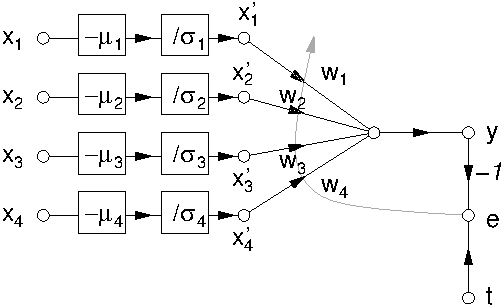
\includegraphics{lms-flow}
\end{center}
\caption{O diagrama de fluxo do discriminador LMS que será empregado na
discriminação elétron-jato.}
\label{fig:lms-flow}
\end{figure}

\section{Processamento Neural}

A Figura~\ref{fig:neuron} contém uma modelagem de um neurônio
genérico. Analogamente ao sistema LMS descrito na Seção~\ref{sec:linear}, os
elementos processadores de uma rede neural, chamados neurônios ou percéptrons,
são ativados por um conjunto de entradas $\overrightarrow{x}$, somadas de
acordo com um sistema linear de ponderação $\overrightarrow{w}$. O diferencial
entre o sistema linear proposto anteriormente e um neurônio está na função de
ativação que conduz o campo induzido $v_p =
\overrightarrow{x}^{T}*\overrightarrow{w}_{p}$ à saída. Enquanto que
no caso do LMS utiliza-se a função identidade, i.e., $y_p = v_p$, no caso de
percéptrons, faz-se uso de uma função não-linear, como por exemplo a função
tangente hiperbólica:

\begin{figure}
\begin{center}
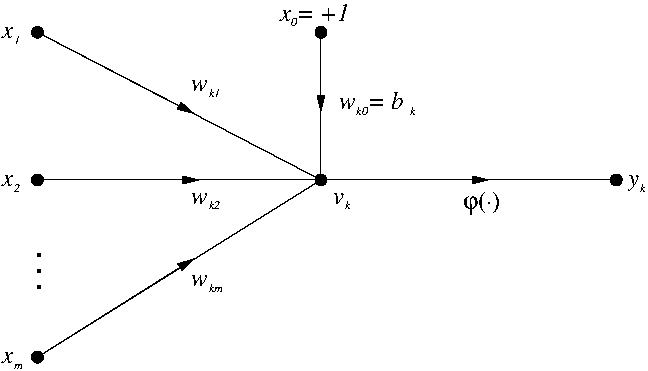
\includegraphics{neuron}
\end{center}
\caption{Grafo de fluxo de sinal de um neurônio artificial.}
\label{fig:neuron}
\end{figure}

\begin{equation}
tanh(v) = \frac{e^v - e^{-v}}{e^v + e^{-v}} = \frac{e^{2v} - 1}{e^{2v} + 1}
\label{eq:tanh}
\end{equation}

Ou a função logística (simplificada):

\begin{equation}
P(v) = \frac{1}{1 + e^{-v}}
\label{eq:logf}
\end{equation}

A razão da escolha de uma função não-linear para a ativação de um campo
induzido pode ser qualificado a partir da seguinte constatação: se o sistema
que se deseja classificar apresenta um comportamento gaussiano, para ambas as
classes, i.e., os momentos de ordem superior a $2$ para ambas as classes são
todos iguais a zero, o classificador ótimo (bayesiano) resume-se a um sistema
linear \cite{haykin}. Naturalmente nota-se que é sempre possível
\textit{aproximar} ou modelar um sistema não-gaussiano em um desta espécie,
tendo-se, por conseqüência, os erros relativos a esta aproximação. De fato,
isto foi realizado na Seção~\ref{sec:linear}, quando escolheu-se utilizar um
classificador linear para separar as quatro variáveis definidas pelo T2Calo.

Se o sistema que se deseja resolver apresenta um comportamento não-gaussiano,
o classificador ótimo não pode ser representado por um classificador
linear. Neste caso, utiliza-se uma função de ativação não-linear para que se
aproxime, de alguma forma, o comportamento não-linear do sistema de interesse.
As funções nas Equações~(\ref{eq:tanh}) e (\ref{eq:logf}) são normalmente
utilizadas por apresentarem amplitude limitada e possuírem derivada
trivialmente calculável. A razão de procurar-se funções com derivadas simples
(e suaves) ficará mais clara adiante, quando se definir o algoritmo de
treinamento. A amplitude limitada pode rapidamente ser verificada como uma
característica de interesse, observando-se que o treinamento de um sistema que
trabalha por aprendizado é muitas vezes executado com a retro-alimentação de
erros. Nesse caso, para evitar oscilações e pontos de ressonância, um sistema
cuja saída seja limitada apresenta natural vantagem se comparado a outro
análogo \cite{haykin}.

Este estudo está focado na utilização de RNA's utilizando percéptrons em
múltiplas camadas (do inglês \eng{Multi-layer perceptrons} ou MLP),
completamente conectadas, sem realimentação e com treinamento baseado tanto na
retropropagação de erros simples (do inglês \eng{back-propagation}) quanto na
retropropagação resiliente (do inglês \eng{resilient
back-propagation}). Introduziremos o processo de treinamento destes sistemas a
seguir.

\subsection{Treinamento por retro-propagação de erros simples}

Para sistemas com apenas uma camada neural, observa-se que, ao buscar-se o
ponto de mínimo da superfície de erro (quadrático), naturalmente otimiza-se o
conjunto de pesos de tal forma que o sistema consiga mapear a entrada nos
alvos de saída. A única restrição do método é que a função de ativação do
campo induzido do neurônio $\varphi(\cdot)$ seja diferenciável.
\cite{rosenblatt}. O problema do treinamento de uma rede MLP é um pouco mais
complexo. Um grafo de fluxo de uma rede MLP completamente conectada pode ser
visto na Figura~\ref{fig:simple-mlp}. Neste caso considera-se que a rede
possui apenas uma camada escondida e apenas um neurônio de saída, o que se
identifica intimamente com os casos de uso que abordaremos. Ainda sim, seria
possível considerar casos com um número maior de neurônios de saída ou com
mais camadas escondidas, generalizando os casos exemplificados aqui.

\begin{figure}
\begin{center}
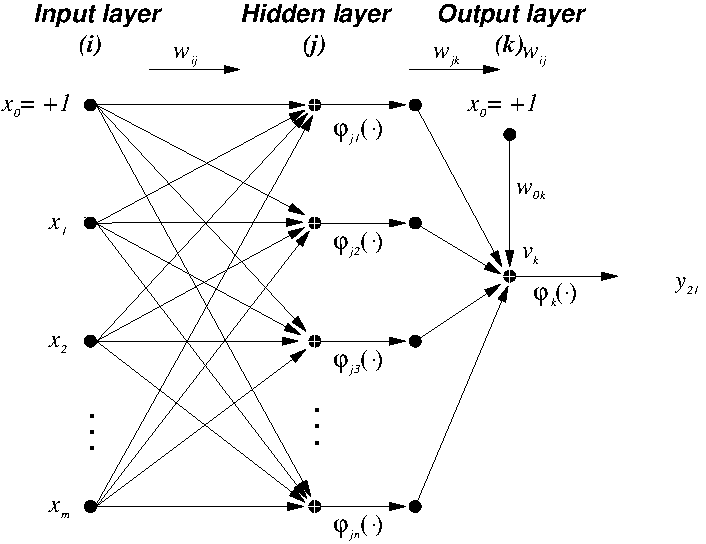
\includegraphics{simple-mlp}
\end{center}
\caption{Modelagem de uma rede MLP, totalmente conectada e sem
retro-propagação de sinal.}
\label{fig:simple-mlp}
\end{figure}

Para o sistema em questão, o mecanismo de treinamento para o neurônio de saída
é idêntico ao treinamento de um percéptron simples, e pode ser facilmente
definido da seguinte forma:

\begin{align}
\text{Definindo o erro como } \mathcal{E}(n) &= \frac{1}{2}e_{k}^{2}(n)
\label{eq:error-def} \\
\text{se observa que } \frac{\partial\mathcal{E}(n)}{\partial
w_{jk}(n)} &= \frac{\partial\mathcal{E}(n)}{\partial e_k(n)} \frac{\partial
e_k(n)}{\partial y_k(n)} \frac{\partial y_k(n)}{\partial v_k(n)}
\frac{\partial v_k(n)}{\partial w_{jk}(n)} \label{eq:partials} \\
\text{ent\~{a}o } \frac{\partial\mathcal{E}(n)}{\partial
w_{jk}(n)} &= e_k(n)(-1)\varphi_{k}'(v_{k}(n))y_{k}(n)
\label{eq:partials-solution} \\
\text{resumindo, } \Delta w_{jk}(n) &=
-\eta\frac{\partial\mathcal{E}(n)}{\partial w_{jk}(n)} = \eta
e_{k}(n)\varphi_{k}'(v_{k}(n))y_{k}(n)
\end{align}

Normalmente, define-se o gradiente local como:

\begin{align}
\delta_k(n) &= - e_k(n)\varphi_{k}'(v_k(n)) \\
\text{e dessa forma, } \Delta w_{jk}(n) &= \eta\delta_k(n)y_{k}(n)
\label{eq:neural-train}
\end{align}

Este sistema de equações segue o princípio definido anteriormente para o LMS,
mas sem assumir nada sobre a função de ativação $\varphi(\cdot)$. Nota-se que
para uma função de ativação onde $y_k(n) = v_k(n)$, recai-se no algoritmo de
treinamento do LMS: $\Delta w_{jk}(n) = \eta e_{j}(n)y_{j}(n)$. Dessa forma, é
possível considerar o LMS como um caso especial de uma rede neural com apenas
uma camada e cuja função de ativação é a função identidade. Nestas equações,
$n$ representa a época ou batelada de treinamento.

O segundo caso de interesse acontece quando o neurônio $j$ está localizado em
uma camada oculta da rede. Neste caso, não existe uma resposta desejada (alvo)
específica para aquele neurônio. Desta forma, tentar-se-á definir o sinal de
erro de um neurônio escondido recursivamente, através da retro-propagação do
erro na saída final da rede em direção ao neurônio desejado. Iniciamos,
intuitivamente, com a definição do gradiente local do neurônio escondido $j$:

\begin{equation}
\delta_j(n) = -\frac{\partial\mathcal{E}(n)}{\partial
v_j(n)} = -\frac{\partial\mathcal{E}(n)}{\partial
y_j(n)}\frac{\partial y_j(n)}{\partial v_j(n)} =
-\frac{\partial\mathcal{E}(n)}{\partial y_j(n)}\varphi_{j}'(v_j(n))
\end{equation}

Tendo em conta que para o caso específico em análise:

\begin{align}
\mathcal{E}(n) &= \frac{1}{2}e_{k}^{2}(n) \\
\text{conclui-se que } \frac{\partial\mathcal{E}(n)}{\partial y_j(n)} &=
e_{k}\frac{\partial e_k(n)}{\partial y_j(n)} = e_{k}\frac{\partial
e_k(n)}{\partial v_k(n)}\frac{\partial v_k(n)}{\partial y_j(n)}
\end{align}

A primeira derivada parcial, $\partial e_k(n)/\partial v_k(n)$, já foi
calculada para o caso do neurônio de saída, na passagem da
Equação~(\ref{eq:partials}) para a
Equação~(\ref{eq:partials-solution}). Utiliza-se a mesma analogia aqui. Para o
cálculo da segunda derivada parcial, pela Figura~\ref{fig:simple-mlp}
deduz-se que:

\begin{align}
v_k(n) &= \sum_{j} w_{jk}(n)y_j(n) \\
\text{e, portanto: } \frac{\partial v_k(n)}{\partial y_j(n)} &= w_{jk}(n)
\end{align}

Assim sendo, o gradiente local do neurônio escondido $j$ assim se define:

\begin{equation}
\delta_j(n) = \varphi_{j}'(v_j(n))\delta_k(n)w_{jk}(n)
\label{eq:local-gradient-hidden}
\end{equation}

Substituindo $\delta_j(n)$ na Equação~(\ref{eq:neural-train}), chega-se a
fórmula de treinamento do neurônio escondido. No caso onde há muitas saídas na
rede, a Equação~(\ref{eq:local-gradient-hidden}) é trivialmente redefinida da
seguinte forma: 

\begin{equation}
\delta_j(n) = \varphi_{j}'(v_j(n))\sum_{k}\delta_k(n)w_{jk}(n)
\label{eq:local-gradient-hidden-multi}
\end{equation}

No caso em que existem múltiplas camadas escondidas, propaga-se recursivamente
o erro em direção à camada de entrada, aplicando-se a
Equação~(\ref{eq:local-gradient-hidden-multi}). 

\subsubsection{Convergência}

O algoritmo de retropropagação usa uma estimativa do gradiente da superfície
de erro no espaço dos pesos. Por esta razão, este sistema possui uma inerente
natureza estocástica e tende a oscilar ao redor da direção de convergência
ótima, ao mínimo da função de erro. Isso acontece pois é difícil antever se
inclinações demasiado bruscas ou suaves em uma das direções da superfície de
erro não influenciarão excessivamente o deslocamento do sistema. Muitas vezes,
a utilização de um amortecimento (ou \emph{momento}) durante o treinamento
pode melhorar a resposta do sistema. Utiliza-se esta técnica para suavizar a
migração das redes em direção ao mínimo da superfície de erro. Outra técnica é
a normalização dos dados de entrada da rede, de forma que se evite que a
diferença de magnitude e variabilidade das componentes de entrada cause
tendências no treinamento neural.

Um problema recorrente no treinamento de redes neurais são mínimos locais, que
podem fazer com que o sistema fique ``preso'' em uma região que não represente
o mínimo global da superfície de erro. Esta característica não é somente mais
uma conseqüência da utilização da estimativa instantânea para definir a
direção de movimentação dos pesos, mas muitas vezes ocorre por dispor-se de
uma quantidade limitada de eventos que representem o fenômeno que se deseja
mapear.

Para que se assegure de que o sistema convirja sempre a um patamar equivalente
de mínimo, deve se realizar um número de experimentos com os mesmos parâmetros
de treinamento e teste para todos os casos de estudo. Em cada teste
inicializam-se os pesos sinápticos a partir de um ponto diferente da
superfície de erro. Desta forma, será possível detetar e avaliar se o problema
em estudo estará sujeito a mínimos locais.

\subsection{Treinamento por retro-propagação de erros resiliente}

Embora a retro-propagação de erros clássica seja um dos mais amplamente
utilizados algoritmos para o treinamento de redes neurais, ela apresenta
problemas fundamentais ligados a sua implementação, dentre os quais a difícil
escolha dos parâmetros de treinamento. Esta parametrização é fortemente
dependente do problema abordado e requer normalmente um certo empirismo para
seu ajuste. A técnica de retro-propagação de erros resiliente (originalmente
descrita em
\cite{rprop}), descreve uma forma de atualizar os pesos sinápticos de uma rede
neural sem retro-alimentação que praticamente remove a necessidade de
parametrização do treinamento. Neste método de treinamento, a atualização do
pesos sinápticos é feita de forma independente do sinal de erro
retro-propagado, dependendo somente da direção do gradiente. Com esta técnica,
o processo de atualização dos pesos sinápticos torna-se independente do valor
do erro retro-propagado, o que, segundo os autores, melhora a dinâmica de
treinamento. O trecho de pseudo-código abaixo descreve o algoritmo:

\begin{alltt}
\textit{Para todos os pesos} \{
  \textit{se} (GradErro(t-1) * GradErro(t) > 0) \textit{então} \{
    Taxa(t) = mínimo(Taxa(t-1) * Incentivo, TaxaMáxima)
    Atualização(t) = -sinal(GradErro(t)) * Taxa(t)
  \}
  \textit{de outra forma, se} (GradErro(t-1) * GradErro(t) < 0) \textit{então} \{
    Taxa(t) = máximo(Taxa(t-1) * Repressão, TaxaMínima)
    Atualização(t) = -Atualização(t-1)
    GradErro(t) = 0
  \}
  \textit{de outra forma, se} (GradErro(t-1) * GradErro(t) = 0) \textit{então} \{
    Atualização(t) = -sinal(GradErro(t)) * Taxa(t-1)
  \}
  Peso(t+1) = Peso(t) + Atualização(t)
\}
\end{alltt}

A atualização funciona da seguinte forma:

\begin{enumerate}
\item Se o gradiente do erro mantiver o mesmo sinal entre duas
atualizações consecutivas da taxa de aprendizado, significa que se encontra em
uma descida na superfície de erro e, para aumentar a velocidade,
multiplica-se a taxa de aprendizado (\texttt{\textit{Taxa(t)}}) por um fator
de incentivo. O valor do fator de incentivo é normalmente igual a $1,2$,
funcionando bem para vários tipos de problemas;
\item Se o gradiente do erro muda de sinal entre duas atualizações, então
perde-se o ponto de mínimo e deve-se:
\begin{enumerate}
\item Retroceder a sinapse do valor do último ajuste (já que foi demasiado);
\item Reprimir a taxa de aprendizado, fazendo com que o próximo passo seja
menos longo, para atingir-se o mínimo. O valor de repressão é normalmente
fixo, igual a $0,5$;
\item Força-se o valor do gradiente a ser zero, de tal forma que na próxima
atualização, o sistema recaia no último caso, onde a atualização do peso não
terá um incentivo;
\end{enumerate}
\item Se o gradiente do erro for zero, então é porque o último passo falhou
o mínimo (zero forçado) e portanto deve-se simplesmente avançar, mantendo-se a
mesma taxa de aprendizagem.
\end{enumerate}

Para evitar \eng{overflows} e \eng{underflows}, institui-se um mínimo e um
máximo para a taxa de aprendizado, em $10^{-6}$ e $50$, respectivamente. A
escolha de fatores de incentivo e repressão dependem, naturalmente, da
superfície de erro na qual se está trabalhando. Superfícies com mais mínimos
locais podem requerem valores de incentivo maiores.

\subsection{Funções de ativação} 

A função de ativação $\varphi(\cdot)$ deve ser diferenciável em toda a
extensão do domínio de interesse. No entanto, para simplificar o cálculo
computacional dos gradientes locais, é habitual a escolha de funções que
possuam um cálculo trival de suas derivadas. Como exemplo, foram citadas as
funções tangente hiperbólica (Equação~\ref{eq:tanh}) e a função logística
simplificada (Equação~\ref{eq:logf}). No caso da função logística:

\begin{align}
\varphi(z) &= \frac{1}{1 + e^{-z}} \\
\text{daí } \varphi'(z) &= \frac{e^{-z}}{[1+e^{-z}]^2}
\end{align}

Levando-se em consideração que para um neurônio genérico $y =
\varphi(v)$, então:

\begin{equation}
\varphi'(v) = \frac{e^{-v}}{[1+e^{-v}]^2} = \frac{1+e^{-v}}{[1+e^{-v}]^2} -
\frac{1}{[1+e^{-v}]^2} = \varphi(v)[1 - \varphi(v)] = y(1-y)
\end{equation}

No caso da tangente hiperbólica, equivalentemente:

\begin{align}
\varphi(z) &= \tanh(z) \\
\varphi'(z) &= \text(sech)^2(z) = 1 - \tanh^2(z) \\
\varphi'(v(n)) &= 1 - \varphi^2(z) = 1-y^2(n)
\end{align}

Estas duas funções de ativação permitem um cálculo absolutamente trivial do
gradiente local, e por esta razão são computacionalmente bastante
eficientes. No contexto deste trabalho utilizaremos a função tangente
hiperbólica como função de ativação dos percéptrons das redes estudadas.

\typeout{ *************** End of file rna.tex *************** }
